\documentclass{standalone}

\usepackage[T1]{fontenc}
\usepackage[utf8]{inputenc}
\usepackage{eulervm}
\usepackage{amsmath}
\usepackage{bm}
\usepackage{tikz}
\usepackage{environ}

\usetikzlibrary{fit}
\usetikzlibrary{patterns}
\usetikzlibrary{arrows}
\usetikzlibrary{positioning}

\usepackage{color}

\definecolor{Comment}{RGB}{97,161,176}

\definecolor{btfGreen}{RGB}{51,160,44}
\definecolor{btfRed}{RGB}{190,60,90}

\definecolor{bleuUni}{RGB}{0, 157, 224}
\definecolor{marronUni}{RGB}{68, 58, 49}
\definecolor{grayMarronUni}{RGB}{60, 60, 60}
\definecolor{grayBleuUni}{RGB}{118, 118, 118}

\definecolor{bluecite}{HTML}{009DE0}

\definecolor{Paired-2}{RGB}{166,206,227}
\definecolor{Paired-1}{RGB}{31,120,180}
\definecolor{Paired-4}{RGB}{178,223,138}
\definecolor{Paired-3}{RGB}{51,160,44}
\definecolor{Paired-6}{RGB}{251,154,153}
\definecolor{Paired-5}{RGB}{227,26,28}
\definecolor{Paired-8}{RGB}{253,191,111}
\definecolor{Paired-7}{RGB}{255,127,0}
\definecolor{Paired-10}{RGB}{202,178,214}
\definecolor{Paired-9}{RGB}{106,61,154}
\definecolor{Paired-12}{RGB}{255,255,153}
\definecolor{Paired-11}{RGB}{177,89,40}
\definecolor{Accent-1}{RGB}{127,201,127}
\definecolor{Accent-2}{RGB}{190,174,212}
\definecolor{Accent-3}{RGB}{253,192,134}
\definecolor{Accent-4}{RGB}{255,255,153}
\definecolor{Accent-5}{RGB}{56,108,176}
\definecolor{Accent-6}{RGB}{240,2,127}
\definecolor{Accent-7}{RGB}{191,91,23}
\definecolor{Accent-8}{RGB}{102,102,102}
\definecolor{Spectral-1}{RGB}{158,1,66}
\definecolor{Spectral-2}{RGB}{213,62,79}
\definecolor{Spectral-3}{RGB}{244,109,67}
\definecolor{Spectral-4}{RGB}{253,174,97}
\definecolor{Spectral-5}{RGB}{254,224,139}
\definecolor{Spectral-6}{RGB}{255,255,191}
\definecolor{Spectral-7}{RGB}{230,245,152}
\definecolor{Spectral-8}{RGB}{171,221,164}
\definecolor{Spectral-9}{RGB}{102,194,165}
\definecolor{Spectral-10}{RGB}{50,136,189}
\definecolor{Spectral-11}{RGB}{94,79,162}
\definecolor{Set1-1}{RGB}{228,26,28}
\definecolor{Set1-2}{RGB}{55,126,184}
\definecolor{Set1-3}{RGB}{77,175,74}
\definecolor{Set1-4}{RGB}{152,78,163}
\definecolor{Set1-5}{RGB}{255,127,0}
\definecolor{Set1-6}{RGB}{255,255,51}
\definecolor{Set1-7}{RGB}{166,86,40}
\definecolor{Set1-8}{RGB}{247,129,191}
\definecolor{Set1-9}{RGB}{153,153,153}
\definecolor{Set2-1}{RGB}{102,194,165}
\definecolor{Set2-2}{RGB}{252,141,98}
\definecolor{Set2-3}{RGB}{141,160,203}
\definecolor{Set2-4}{RGB}{231,138,195}
\definecolor{Set2-5}{RGB}{166,216,84}
\definecolor{Set2-6}{RGB}{255,217,47}
\definecolor{Set2-7}{RGB}{229,196,148}
\definecolor{Set2-8}{RGB}{179,179,179}
\definecolor{Dark2-1}{RGB}{27,158,119}
\definecolor{Dark2-2}{RGB}{217,95,2}
\definecolor{Dark2-3}{RGB}{117,112,179}
\definecolor{Dark2-4}{RGB}{231,41,138}
\definecolor{Dark2-5}{RGB}{102,166,30}
\definecolor{Dark2-6}{RGB}{230,171,2}
\definecolor{Dark2-7}{RGB}{166,118,29}
\definecolor{Dark2-8}{RGB}{102,102,102}
\definecolor{Reds-1}{RGB}{255,245,240}
\definecolor{Reds-2}{RGB}{254,224,210}
\definecolor{Reds-3}{RGB}{252,187,161}
\definecolor{Reds-4}{RGB}{252,146,114}
\definecolor{Reds-5}{RGB}{251,106,74}
\definecolor{Reds-6}{RGB}{239,59,44}
\definecolor{Reds-7}{RGB}{203,24,29}
\definecolor{Reds-8}{RGB}{165,15,21}
\definecolor{Reds-9}{RGB}{103,0,13}
\definecolor{Greens-1}{RGB}{247,252,245}
\definecolor{Greens-2}{RGB}{229,245,224}
\definecolor{Greens-3}{RGB}{199,233,192}
\definecolor{Greens-4}{RGB}{161,217,155}
\definecolor{Greens-5}{RGB}{116,196,118}
\definecolor{Greens-6}{RGB}{65,171,93}
\definecolor{Greens-7}{RGB}{35,139,69}
\definecolor{Greens-8}{RGB}{0,109,44}
\definecolor{Greens-9}{RGB}{0,68,27}
\definecolor{Blues-1}{RGB}{247,251,255}
\definecolor{Blues-2}{RGB}{222,235,247}
\definecolor{Blues-3}{RGB}{198,219,239}
\definecolor{Blues-4}{RGB}{158,202,225}
\definecolor{Blues-5}{RGB}{107,174,214}
\definecolor{Blues-6}{RGB}{66,146,198}
\definecolor{Blues-7}{RGB}{33,113,181}
\definecolor{Blues-8}{RGB}{8,81,156}
\definecolor{Blues-9}{RGB}{8,48,107}


\begin{document}
  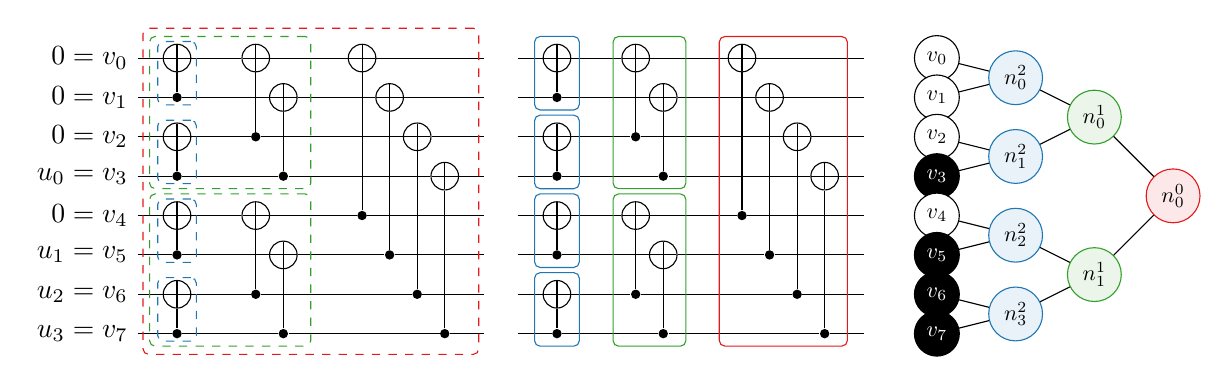
\begin{tikzpicture}%[scale=\tikzscale]

  \tikzset{XOR/.style={draw,circle, minimum height=0.35cm,append after command={
          [shorten >=\pgflinewidth, shorten <=\pgflinewidth,]
          (\tikzlastnode.north) edge (\tikzlastnode.south)
          (\tikzlastnode.east) edge (\tikzlastnode.west)
          }
      }
  }

  \tikzset{DOT/.style={circle,fill,inner sep=1.2pt} }

  \newcommand\startx{0.0}
  \newcommand\startyg{0}
  \newcommand\sed{0.50}
  \newcommand\stasep{1.00}
  \newcommand\xorsep{0.35}

  \renewcommand\startyg{0.0}


  \node[XOR] (g3_x0) at (\startx,                 \startyg+1.75)       {};
  \node      (g3_e0) at (\startx,                 \startyg+1.25) [DOT] {};

  \node[XOR] (g3_x1) at (\startx,                 \startyg+0.75)       {};
  \node      (g3_e1) at (\startx,                 \startyg+0.25) [DOT] {};

  % ---

  \node[XOR] (g3_x2) at (\startx+\stasep,         \startyg+1.75)       {};
  \node[XOR] (g3_x3) at (\startx+\stasep+\xorsep, \startyg+1.25)       {};

  \node      (g3_e2) at (\startx+\stasep,         \startyg+0.75) [DOT] {};
  \node      (g3_e3) at (\startx+\stasep+\xorsep, \startyg+0.25) [DOT] {};

  % -----

  \node[XOR] (g3_x4) at (\startx,                 \startyg-0.25)       {};
  \node      (g3_e4) at (\startx,                 \startyg-0.75) [DOT] {};

  \node[XOR] (g3_x5) at (\startx,                 \startyg-1.25)       {};
  \node      (g3_e5) at (\startx,                 \startyg-1.75) [DOT] {};

  % ---

  \node[XOR] (g3_x6) at (\startx+\stasep,         \startyg-0.25)       {};
  \node[XOR] (g3_x7) at (\startx+\stasep+\xorsep, \startyg-0.75)       {};

  \node      (g3_e6) at (\startx+\stasep,         \startyg-1.25) [DOT] {};
  \node      (g3_e7) at (\startx+\stasep+\xorsep, \startyg-1.75) [DOT] {};

  % ----------

  \node[XOR] (g3_x8)  at (\startx+\stasep+\stasep+\xorsep,                         \startyg+1.75)       {};
  \node[XOR] (g3_x9)  at (\startx+\stasep+\stasep+\xorsep+\xorsep,                 \startyg+1.25)       {};
  \node[XOR] (g3_x10) at (\startx+\stasep+\stasep+\xorsep+\xorsep+\xorsep,         \startyg+0.75)       {};
  \node[XOR] (g3_x11) at (\startx+\stasep+\stasep+\xorsep+\xorsep+\xorsep+\xorsep, \startyg+0.25)       {};

  \node      (g3_e8)  at (\startx+\stasep+\stasep+\xorsep,                         \startyg-0.25) [DOT] {};
  \node      (g3_e9)  at (\startx+\stasep+\stasep+\xorsep+\xorsep,                 \startyg-0.75) [DOT] {};
  \node      (g3_e10) at (\startx+\stasep+\stasep+\xorsep+\xorsep+\xorsep,         \startyg-1.25) [DOT] {};
  \node      (g3_e11) at (\startx+\stasep+\stasep+\xorsep+\xorsep+\xorsep+\xorsep, \startyg-1.75) [DOT] {};

  \draw[-,>=latex] (\startx-\sed, \startyg+1.75) node[left] {$0 = v_0$} -- (g3_x0);
  \draw[-,>=latex] (\startx-\sed, \startyg+1.25) node[left] {$0 = v_1$} -- (g3_e0);
  \draw[-,>=latex] (g3_x0)                       -- (g3_e0);
  \draw[-,>=latex] (g3_x0)                       -- (g3_x2);
  \draw[-,>=latex] (g3_e0)                       -- (g3_x3);

  \draw[-,>=latex] (\startx-\sed, \startyg+0.75) node[left] {$0 = v_2$} -- (g3_x1);
  \draw[-,>=latex] (\startx-\sed, \startyg+0.25) node[left] {$u_0 = v_3$} -- (g3_e1);
  \draw[-,>=latex] (g3_x1)                       -- (g3_e1);
  \draw[-,>=latex] (g3_x1)                       -- (g3_e2);
  \draw[-,>=latex] (g3_e1)                       -- (g3_e3);
  \draw[-,>=latex] (g3_e2)                       -- (g3_x2);
  \draw[-,>=latex] (g3_e3)                       -- (g3_x3);
  \draw[-,>=latex] (g3_x2)                       -- (g3_x8);
  \draw[-,>=latex] (g3_x3)                       -- (g3_x9);
  \draw[-,>=latex] (g3_e2)                       -- (g3_x10);
  \draw[-,>=latex] (g3_e3)                       -- (g3_x11);

  \draw[-,>=latex] (\startx-\sed, \startyg-0.25) node[left] {$0 = v_4$} -- (g3_x4);
  \draw[-,>=latex] (\startx-\sed, \startyg-0.75) node[left] {$u_1 = v_5$} -- (g3_e4);
  \draw[-,>=latex] (g3_x4)                       -- (g3_e4);
  \draw[-,>=latex] (g3_x4)                       -- (g3_x6);
  \draw[-,>=latex] (g3_e4)                       -- (g3_x7);

  \draw[-,>=latex] (\startx-\sed, \startyg-1.25) node[left] {$u_2 = v_6$} -- (g3_x5);
  \draw[-,>=latex] (\startx-\sed, \startyg-1.75) node[left] {$u_3 = v_7$} -- (g3_e5);
  \draw[-,>=latex] (g3_x5)                       -- (g3_e5);
  \draw[-,>=latex] (g3_x5)                       -- (g3_e6);
  \draw[-,>=latex] (g3_e5)                       -- (g3_e7);
  \draw[-,>=latex] (g3_e6)                       -- (g3_x6);
  \draw[-,>=latex] (g3_e7)                       -- (g3_x7);
  \draw[-,>=latex] (g3_x6)                       -- (g3_e8);
  \draw[-,>=latex] (g3_x7)                       -- (g3_e9);
  \draw[-,>=latex] (g3_e6)                       -- (g3_e10);
  \draw[-,>=latex] (g3_e7)                       -- (g3_e11);

  \draw [-,>=latex] (g3_e8)                      -- (g3_x8);
  \draw [-,>=latex] (g3_e9)                      -- (g3_x9);
  \draw [-,>=latex] (g3_e10)                     -- (g3_x10);
  \draw [-,>=latex] (g3_e11)                     -- (g3_x11);

  % \draw[-,>=latex] (\startx+\stasep+\stasep+\xorsep+\xorsep+\xorsep+\sed, \startyg+1.75) node[right] {$c_0 = v_0 \oplus v_1 \oplus v_2 \oplus v_3 \oplus v_4 \oplus v_5 \oplus v_6 \oplus v_7$} -- (g3_x8);
  \draw[-,>=latex] (\startx+\stasep+\stasep+\xorsep+\xorsep+\xorsep+\xorsep+\sed, \startyg+1.75) -- (g3_x8);
  \draw[-,>=latex] (\startx+\stasep+\stasep+\xorsep+\xorsep+\xorsep+\xorsep+\sed, \startyg+1.25) -- (g3_x9);
  \draw[-,>=latex] (\startx+\stasep+\stasep+\xorsep+\xorsep+\xorsep+\xorsep+\sed, \startyg+0.75) -- (g3_x10);
  \draw[-,>=latex] (\startx+\stasep+\stasep+\xorsep+\xorsep+\xorsep+\xorsep+\sed, \startyg+0.25) -- (g3_x11);
  \draw[-,>=latex] (\startx+\stasep+\stasep+\xorsep+\xorsep+\xorsep+\xorsep+\sed, \startyg-0.25) -- (g3_e8);
  \draw[-,>=latex] (\startx+\stasep+\stasep+\xorsep+\xorsep+\xorsep+\xorsep+\sed, \startyg-0.75) -- (g3_e9);
  \draw[-,>=latex] (\startx+\stasep+\stasep+\xorsep+\xorsep+\xorsep+\xorsep+\sed, \startyg-1.25) -- (g3_e10);
  \draw[-,>=latex] (\startx+\stasep+\stasep+\xorsep+\xorsep+\xorsep+\xorsep+\sed, \startyg-1.75) -- (g3_e11);

  \node[draw=Paired-1, scale=0.82, rounded corners=2pt, dashed, fit=(g3_x0) (g3_e0)] (g3_l3_1) {};
  \node[draw=Paired-1, scale=0.82, rounded corners=2pt, dashed, fit=(g3_x1) (g3_e1)] (g2_l3_2) {};
  \node[draw=Paired-1, scale=0.82, rounded corners=2pt, dashed, fit=(g3_x4) (g3_e4)] (g3_l3_3) {};
  \node[draw=Paired-1, scale=0.82, rounded corners=2pt, dashed, fit=(g3_x5) (g3_e5)] (g2_l3_4) {};

  \node[draw=Paired-3, scale=0.975, minimum width=2.1cm, rounded corners=2pt, dashed, fit=(g3_x0) (g3_x2) (g3_x3) (g3_e2) (g3_e3)] (g3_l1_1) {};
  \node[draw=Paired-3, scale=0.975, minimum width=2.1cm, rounded corners=2pt, dashed, fit=(g3_x4) (g3_x6) (g3_x7) (g3_e6) (g3_e7)] (g3_l1_2) {};

  \node[draw=Paired-5, scale=1.040, minimum width=4.1cm, rounded corners=2pt, dashed, fit=(g3_x0) (g3_e5) (g3_x8) (g3_x11) (g3_e8) (g3_e11)] (g3_l1_1) {};


  % ---------------------------------------------------------------------------
  % ---------------------------------------------------------------------------
  % ---------------------------------------------------------------------------

  \renewcommand\startx{4.825}

  \node[XOR] (g3_x0) at (\startx,                 \startyg+1.75)       {};
  \node      (g3_e0) at (\startx,                 \startyg+1.25) [DOT] {};

  \node[XOR] (g3_x1) at (\startx,                 \startyg+0.75)       {};
  \node      (g3_e1) at (\startx,                 \startyg+0.25) [DOT] {};

  % ---

  \node[XOR] (g3_x2) at (\startx+\stasep,         \startyg+1.75)       {};
  \node[XOR] (g3_x3) at (\startx+\stasep+\xorsep, \startyg+1.25)       {};

  \node      (g3_e2) at (\startx+\stasep,         \startyg+0.75) [DOT] {};
  \node      (g3_e3) at (\startx+\stasep+\xorsep, \startyg+0.25) [DOT] {};

  % -----

  \node[XOR] (g3_x4) at (\startx,                 \startyg-0.25)       {};
  \node      (g3_e4) at (\startx,                 \startyg-0.75) [DOT] {};

  \node[XOR] (g3_x5) at (\startx,                 \startyg-1.25)       {};
  \node      (g3_e5) at (\startx,                 \startyg-1.75) [DOT] {};

  % ---

  \node[XOR] (g3_x6) at (\startx+\stasep,         \startyg-0.25)       {};
  \node[XOR] (g3_x7) at (\startx+\stasep+\xorsep, \startyg-0.75)       {};

  \node      (g3_e6) at (\startx+\stasep,         \startyg-1.25) [DOT] {};
  \node      (g3_e7) at (\startx+\stasep+\xorsep, \startyg-1.75) [DOT] {};

  % ----------

  \node[XOR] (g3_x8)  at (\startx+\stasep+\stasep+\xorsep,                         \startyg+1.75)       {};
  \node[XOR] (g3_x9)  at (\startx+\stasep+\stasep+\xorsep+\xorsep,                 \startyg+1.25)       {};
  \node[XOR] (g3_x10) at (\startx+\stasep+\stasep+\xorsep+\xorsep+\xorsep,         \startyg+0.75)       {};
  \node[XOR] (g3_x11) at (\startx+\stasep+\stasep+\xorsep+\xorsep+\xorsep+\xorsep, \startyg+0.25)       {};

  \node      (g3_e8)  at (\startx+\stasep+\stasep+\xorsep,                         \startyg-0.25) [DOT] {};
  \node      (g3_e9)  at (\startx+\stasep+\stasep+\xorsep+\xorsep,                 \startyg-0.75) [DOT] {};
  \node      (g3_e10) at (\startx+\stasep+\stasep+\xorsep+\xorsep+\xorsep,         \startyg-1.25) [DOT] {};
  \node      (g3_e11) at (\startx+\stasep+\stasep+\xorsep+\xorsep+\xorsep+\xorsep, \startyg-1.75) [DOT] {};

  \draw[-,>=latex] (\startx-\sed, \startyg+1.75) -- (g3_x0);
  \draw[-,>=latex] (\startx-\sed, \startyg+1.25) -- (g3_e0);
  \draw[-,>=latex] (g3_x0)                       -- (g3_e0);
  \draw[-,>=latex] (g3_x0)                       -- (g3_x2);
  \draw[-,>=latex] (g3_e0)                       -- (g3_x3);

  \draw[-,>=latex] (\startx-\sed, \startyg+0.75) -- (g3_x1);
  \draw[-,>=latex] (\startx-\sed, \startyg+0.25) -- (g3_e1);
  \draw[-,>=latex] (g3_x1)                       -- (g3_e1);
  \draw[-,>=latex] (g3_x1)                       -- (g3_e2);
  \draw[-,>=latex] (g3_e1)                       -- (g3_e3);
  \draw[-,>=latex] (g3_e2)                       -- (g3_x2);
  \draw[-,>=latex] (g3_e3)                       -- (g3_x3);
  \draw[-,>=latex] (g3_x2)                       -- (g3_x8);
  \draw[-,>=latex] (g3_x3)                       -- (g3_x9);
  \draw[-,>=latex] (g3_e2)                       -- (g3_x10);
  \draw[-,>=latex] (g3_e3)                       -- (g3_x11);

  \draw[-,>=latex] (\startx-\sed, \startyg-0.25) -- (g3_x4);
  \draw[-,>=latex] (\startx-\sed, \startyg-0.75) -- (g3_e4);
  \draw[-,>=latex] (g3_x4)                       -- (g3_e4);
  \draw[-,>=latex] (g3_x4)                       -- (g3_x6);
  \draw[-,>=latex] (g3_e4)                       -- (g3_x7);

  \draw[-,>=latex] (\startx-\sed, \startyg-1.25) -- (g3_x5);
  \draw[-,>=latex] (\startx-\sed, \startyg-1.75) -- (g3_e5);
  \draw[-,>=latex] (g3_x5)                       -- (g3_e5);
  \draw[-,>=latex] (g3_x5)                       -- (g3_e6);
  \draw[-,>=latex] (g3_e5)                       -- (g3_e7);
  \draw[-,>=latex] (g3_e6)                       -- (g3_x6);
  \draw[-,>=latex] (g3_e7)                       -- (g3_x7);
  \draw[-,>=latex] (g3_x6)                       -- (g3_e8);
  \draw[-,>=latex] (g3_x7)                       -- (g3_e9);
  \draw[-,>=latex] (g3_e6)                       -- (g3_e10);
  \draw[-,>=latex] (g3_e7)                       -- (g3_e11);

  \draw [-,>=latex] (g3_e8)                      -- (g3_x8);
  \draw [-,>=latex] (g3_e9)                      -- (g3_x9);
  \draw [-,>=latex] (g3_e10)                     -- (g3_x10);
  \draw [-,>=latex] (g3_e11)                     -- (g3_x11);

  \draw[-,>=latex] (\startx+\stasep+\stasep+\xorsep+\xorsep+\xorsep+\xorsep+\sed, \startyg+1.75) -- (g3_x8);
  \draw[-,>=latex] (\startx+\stasep+\stasep+\xorsep+\xorsep+\xorsep+\xorsep+\sed, \startyg+1.25) -- (g3_x9);
  \draw[-,>=latex] (\startx+\stasep+\stasep+\xorsep+\xorsep+\xorsep+\xorsep+\sed, \startyg+0.75) -- (g3_x10);
  \draw[-,>=latex] (\startx+\stasep+\stasep+\xorsep+\xorsep+\xorsep+\xorsep+\sed, \startyg+0.25) -- (g3_x11);
  \draw[-,>=latex] (\startx+\stasep+\stasep+\xorsep+\xorsep+\xorsep+\xorsep+\sed, \startyg-0.25) -- (g3_e8);
  \draw[-,>=latex] (\startx+\stasep+\stasep+\xorsep+\xorsep+\xorsep+\xorsep+\sed, \startyg-0.75) -- (g3_e9);
  \draw[-,>=latex] (\startx+\stasep+\stasep+\xorsep+\xorsep+\xorsep+\xorsep+\sed, \startyg-1.25) -- (g3_e10);
  \draw[-,>=latex] (\startx+\stasep+\stasep+\xorsep+\xorsep+\xorsep+\xorsep+\sed, \startyg-1.75) -- (g3_e11);

  \node[draw=Paired-1, scale=0.95, rounded corners=2pt, fit=(g3_x0) (g3_e0)] (g3_l3_1) {};
  \node[draw=Paired-1, scale=0.95, rounded corners=2pt, fit=(g3_x1) (g3_e1)] (g2_l3_2) {};
  \node[draw=Paired-1, scale=0.95, rounded corners=2pt, fit=(g3_x4) (g3_e4)] (g3_l3_3) {};
  \node[draw=Paired-1, scale=0.95, rounded corners=2pt, fit=(g3_x5) (g3_e5)] (g2_l3_4) {};

  \node[draw=Paired-3, scale=0.975, rounded corners=2pt, fit=(g3_x2) (g3_x3) (g3_e2) (g3_e3)] (g3_l1_1) {};
  \node[draw=Paired-3, scale=0.975, rounded corners=2pt, fit=(g3_x6) (g3_x7) (g3_e6) (g3_e7)] (g3_l1_2) {};

  \node[draw=Paired-5, scale=0.987, rounded corners=2pt, fit=(g3_x8) (g3_x11) (g3_e8) (g3_e11)] (g3_l1_1) {};

  % ---------------------------------------------------------------------------
  % ---------------------------------------------------------------------------
  % ---------------------------------------------------------------------------

  \renewcommand\startx{9.65}

  \node[draw=black, fill=white, text=black, circle, minimum width=0.5cm, scale=0.8] (g3_n0) at (\startx, \startyg+1.75) {$v_0$};
  \node[draw=black, fill=white, text=black, circle, minimum width=0.3cm, scale=0.8] (g3_n1) at (\startx, \startyg+1.25) {$v_1$};
  \node[draw=black, fill=white, text=black, circle, minimum width=0.3cm, scale=0.8] (g3_n2) at (\startx, \startyg+0.75) {$v_2$};
  \node[draw=black, fill=black, text=white, circle, minimum width=0.3cm, scale=0.8] (g3_n3) at (\startx, \startyg+0.25) {$v_3$};
  \node[draw=black, fill=white, text=black, circle, minimum width=0.3cm, scale=0.8] (g3_n4) at (\startx, \startyg-0.25) {$v_4$};
  \node[draw=black, fill=black, text=white, circle, minimum width=0.3cm, scale=0.8] (g3_n5) at (\startx, \startyg-0.75) {$v_5$};
  \node[draw=black, fill=black, text=white, circle, minimum width=0.3cm, scale=0.8] (g3_n6) at (\startx, \startyg-1.25) {$v_6$};
  \node[draw=black, fill=black, text=white, circle, minimum width=0.3cm, scale=0.8] (g3_n7) at (\startx, \startyg-1.75) {$v_7$};

  \node[draw=Paired-1, fill=Paired-1!10, circle, minimum width=0.5cm, scale=0.8] (g3_n8) at (\startx+\stasep, \startyg+1.5) {$n_0^2$};
  \node[draw=Paired-1, fill=Paired-1!10, circle, minimum width=0.5cm, scale=0.8] (g3_n9) at (\startx+\stasep, \startyg+0.5) {$n_1^2$};
  \node[draw=Paired-1, fill=Paired-1!10, circle, minimum width=0.5cm, scale=0.8] (g3_n10) at (\startx+\stasep, \startyg-0.5) {$n_2^2$};
  \node[draw=Paired-1, fill=Paired-1!10, circle, minimum width=0.5cm, scale=0.8] (g3_n11) at (\startx+\stasep, \startyg-1.5) {$n_3^2$};

  \node[draw=Paired-3, fill=Paired-3!10, circle, minimum width=0.5cm, scale=0.8] (g3_n12) at (\startx+\stasep+\stasep, \startyg+1.00) {$n_0^1$};
  \node[draw=Paired-3, fill=Paired-3!10, circle, minimum width=0.5cm, scale=0.8] (g3_n13) at (\startx+\stasep+\stasep, \startyg-1.00) {$n_1^1$};

  \node[draw=Paired-5, fill=Paired-5!10, circle, minimum width=0.5cm, scale=0.8] (g3_n14) at (\startx+\stasep+\stasep+\stasep, \startyg+0.00) {$n_0^0$};

  \draw [-,>=latex] (g3_n14) -- (g3_n13);
  \draw [-,>=latex] (g3_n14) -- (g3_n12);
  \draw [-,>=latex] (g3_n13) -- (g3_n11);
  \draw [-,>=latex] (g3_n13) -- (g3_n10);
  \draw [-,>=latex] (g3_n12) -- (g3_n9);
  \draw [-,>=latex] (g3_n12) -- (g3_n8);
  \draw [-,>=latex] (g3_n11) -- (g3_n7);
  \draw [-,>=latex] (g3_n11) -- (g3_n6);
  \draw [-,>=latex] (g3_n10) -- (g3_n5);
  \draw [-,>=latex] (g3_n10) -- (g3_n4);
  \draw [-,>=latex] (g3_n9)  -- (g3_n3);
  \draw [-,>=latex] (g3_n9)  -- (g3_n2);
  \draw [-,>=latex] (g3_n8)  -- (g3_n1);
  \draw [-,>=latex] (g3_n8)  -- (g3_n0);

  \end{tikzpicture}
\end{document}